\chapter{Problema}

\section{Definirea problemei}

Problema pe care am încercat să o rezolv constă în primul rând în a urmări cu acuratețe ochii utilizatorului, astfel încât cursorul să poată fi mișcat în concordanță cu privirea acestuia.
Această problemă face parte dintr-o gamă mai largă de probleme de \emph{Viziune Computerizată} (în engleză \emph{Computer Vision}), mai exact \emph{Urmărirea ochilor}, după cum a fost menționat și în introducere.
Conform \cite{eye_tracking}, urmărirea ochilor este ``procesul de măsurare a punctului de privire (unde se uită o persoană) sau a mișcării unui ochi relativ la cap''.\footnote{Textul original este din engleză: ``the process of measuring either the point of gaze (where one is looking) or the motion of an eye relative to the head''}

Tehnicile de ultimă oră (\emph{state of the art}) de a rezolva această problemă se bazează pe \emph{Inteligența Artificială} și sunt, mai exact, tehnici de \emph{Învățare Automată}.
\cite{liviu_ciortuz_ml} explică în termeni foarte simpli acest subdomeniu al informaticii: ``Învățarea Automată este programare bazată pe date''\footnote{Traducere liberă; text original: ``ML is data-driven programming''}.
Învățarea poate fi la rândul ei supervizată, semi-supervizată sau nesupervizată, aceste tehnici încearcând să prezică, să producă, să generalizeze niște rezultate pe baza unor exemple sau a unor relații dintr-o mulțime de date deja cunoscută.
Diferența cheie între acestea constă în structura acestei mulțimi de date, structură care la rândul ei influențează abordările de învățare.

Această ramură a Inteligenței Artificiale poate fi mai departe divizată în mai multe secțiuni, una dintre ele fiind \emph{Invățarea Profundă}.
Ea se preocupă, printre altele, de procesarea și analizarea imaginilor prin folosirea unor \emph{arhitecturi profunde} bazate pe \emph{rețele neuronale}.
Învățarea poate fi la rândul ei supervizată, semi-supervizată sau nesupervizată.
În termeni simpli, aceste tehnici încearcă să prezică sau să producă un rezultat pe baza unor exemple sau a unor relații între datele care trebuiesc procesate.

Am formulat problema ca una de învățare profundă supervizată, care presupune cunoașterea unei mulțimi de date
$$D = \{(i, o) | i \in I, o \in O\}$$
unde $I$ reprezintă mulțimea exemplelor pe care le avem iar $O$ mulțimea rezultatelor, a \emph{adevărurilor de bază} deja cunoscute, pe care trebuie să le putem reproduce și prezice corect pentru imagini noi.

Am definit obiectivul ca fiind acela de a prezice zona de pe ecran pe care o privește utilizatorul.
Pentru acest lucru am plasat o ``grilă'' pe ecran și am numerotat fiecare celulă corespunzătoare.
Am experimentat cu mai multe dimensiuni ale grilei, precum 2x2, 3x2 și 4x4.

\begin{figure}[H]
    \centering
    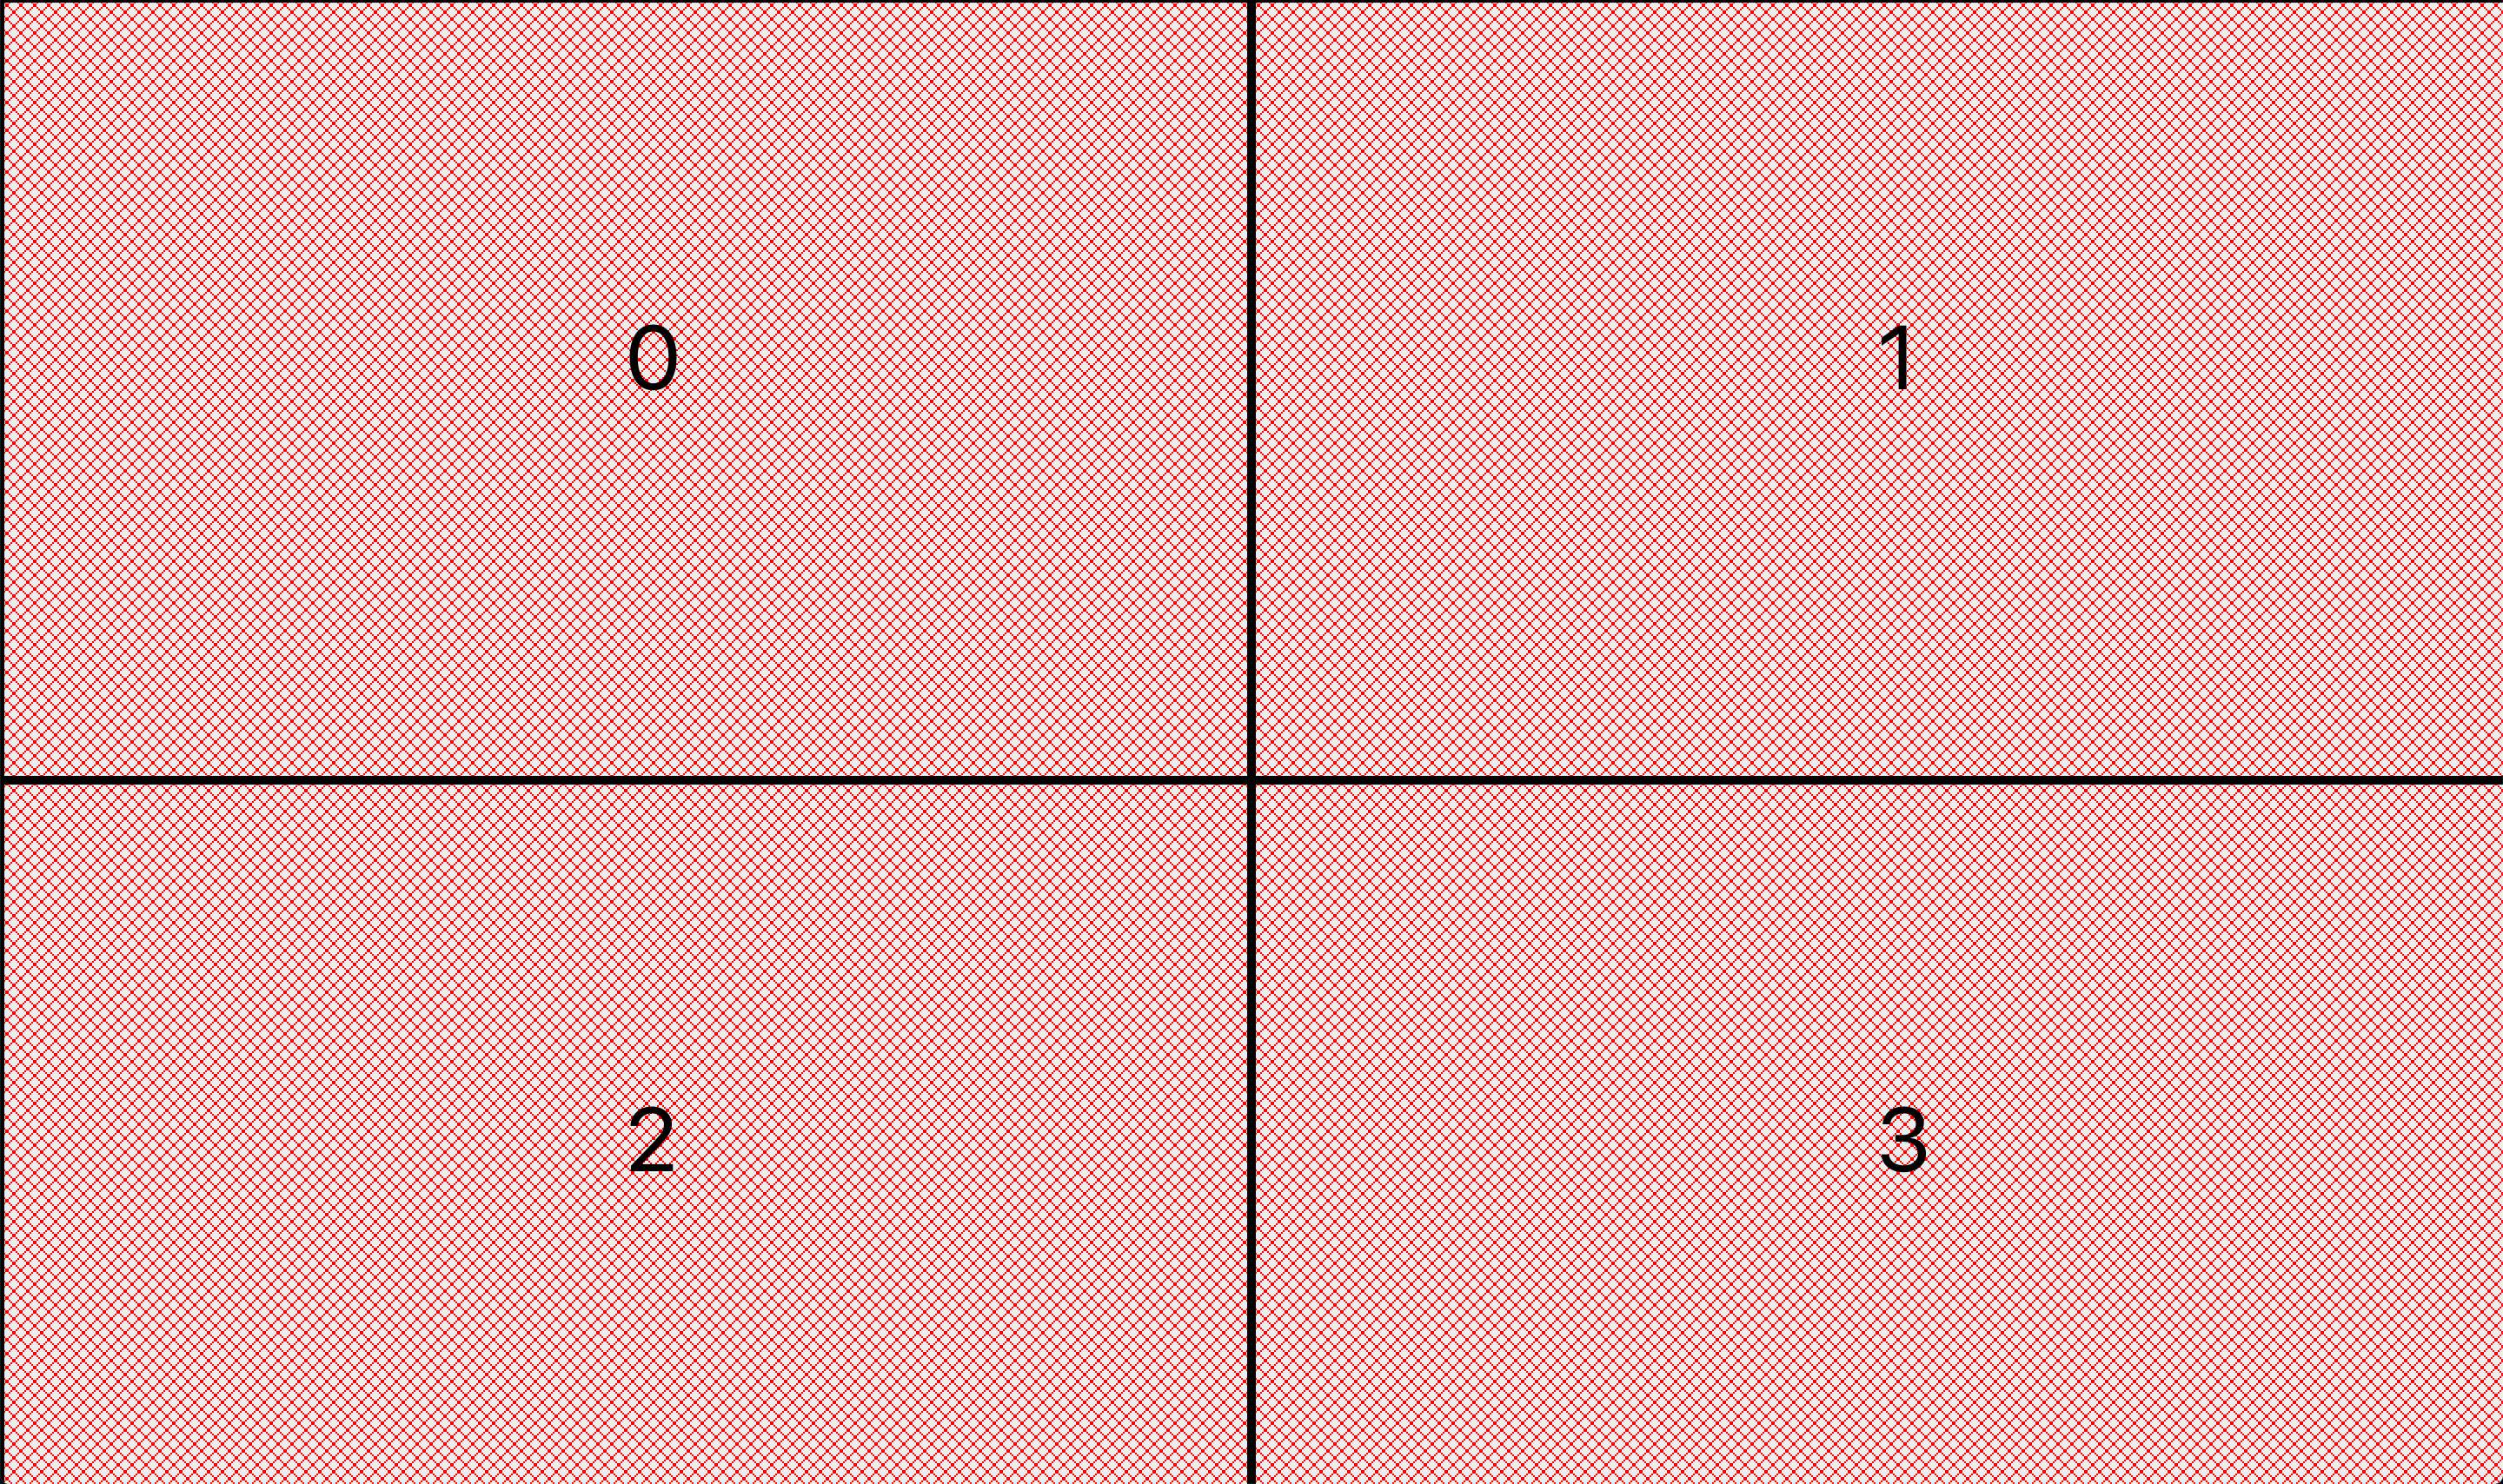
\includegraphics[width=0.32\textwidth]{grid_2_2.png}
    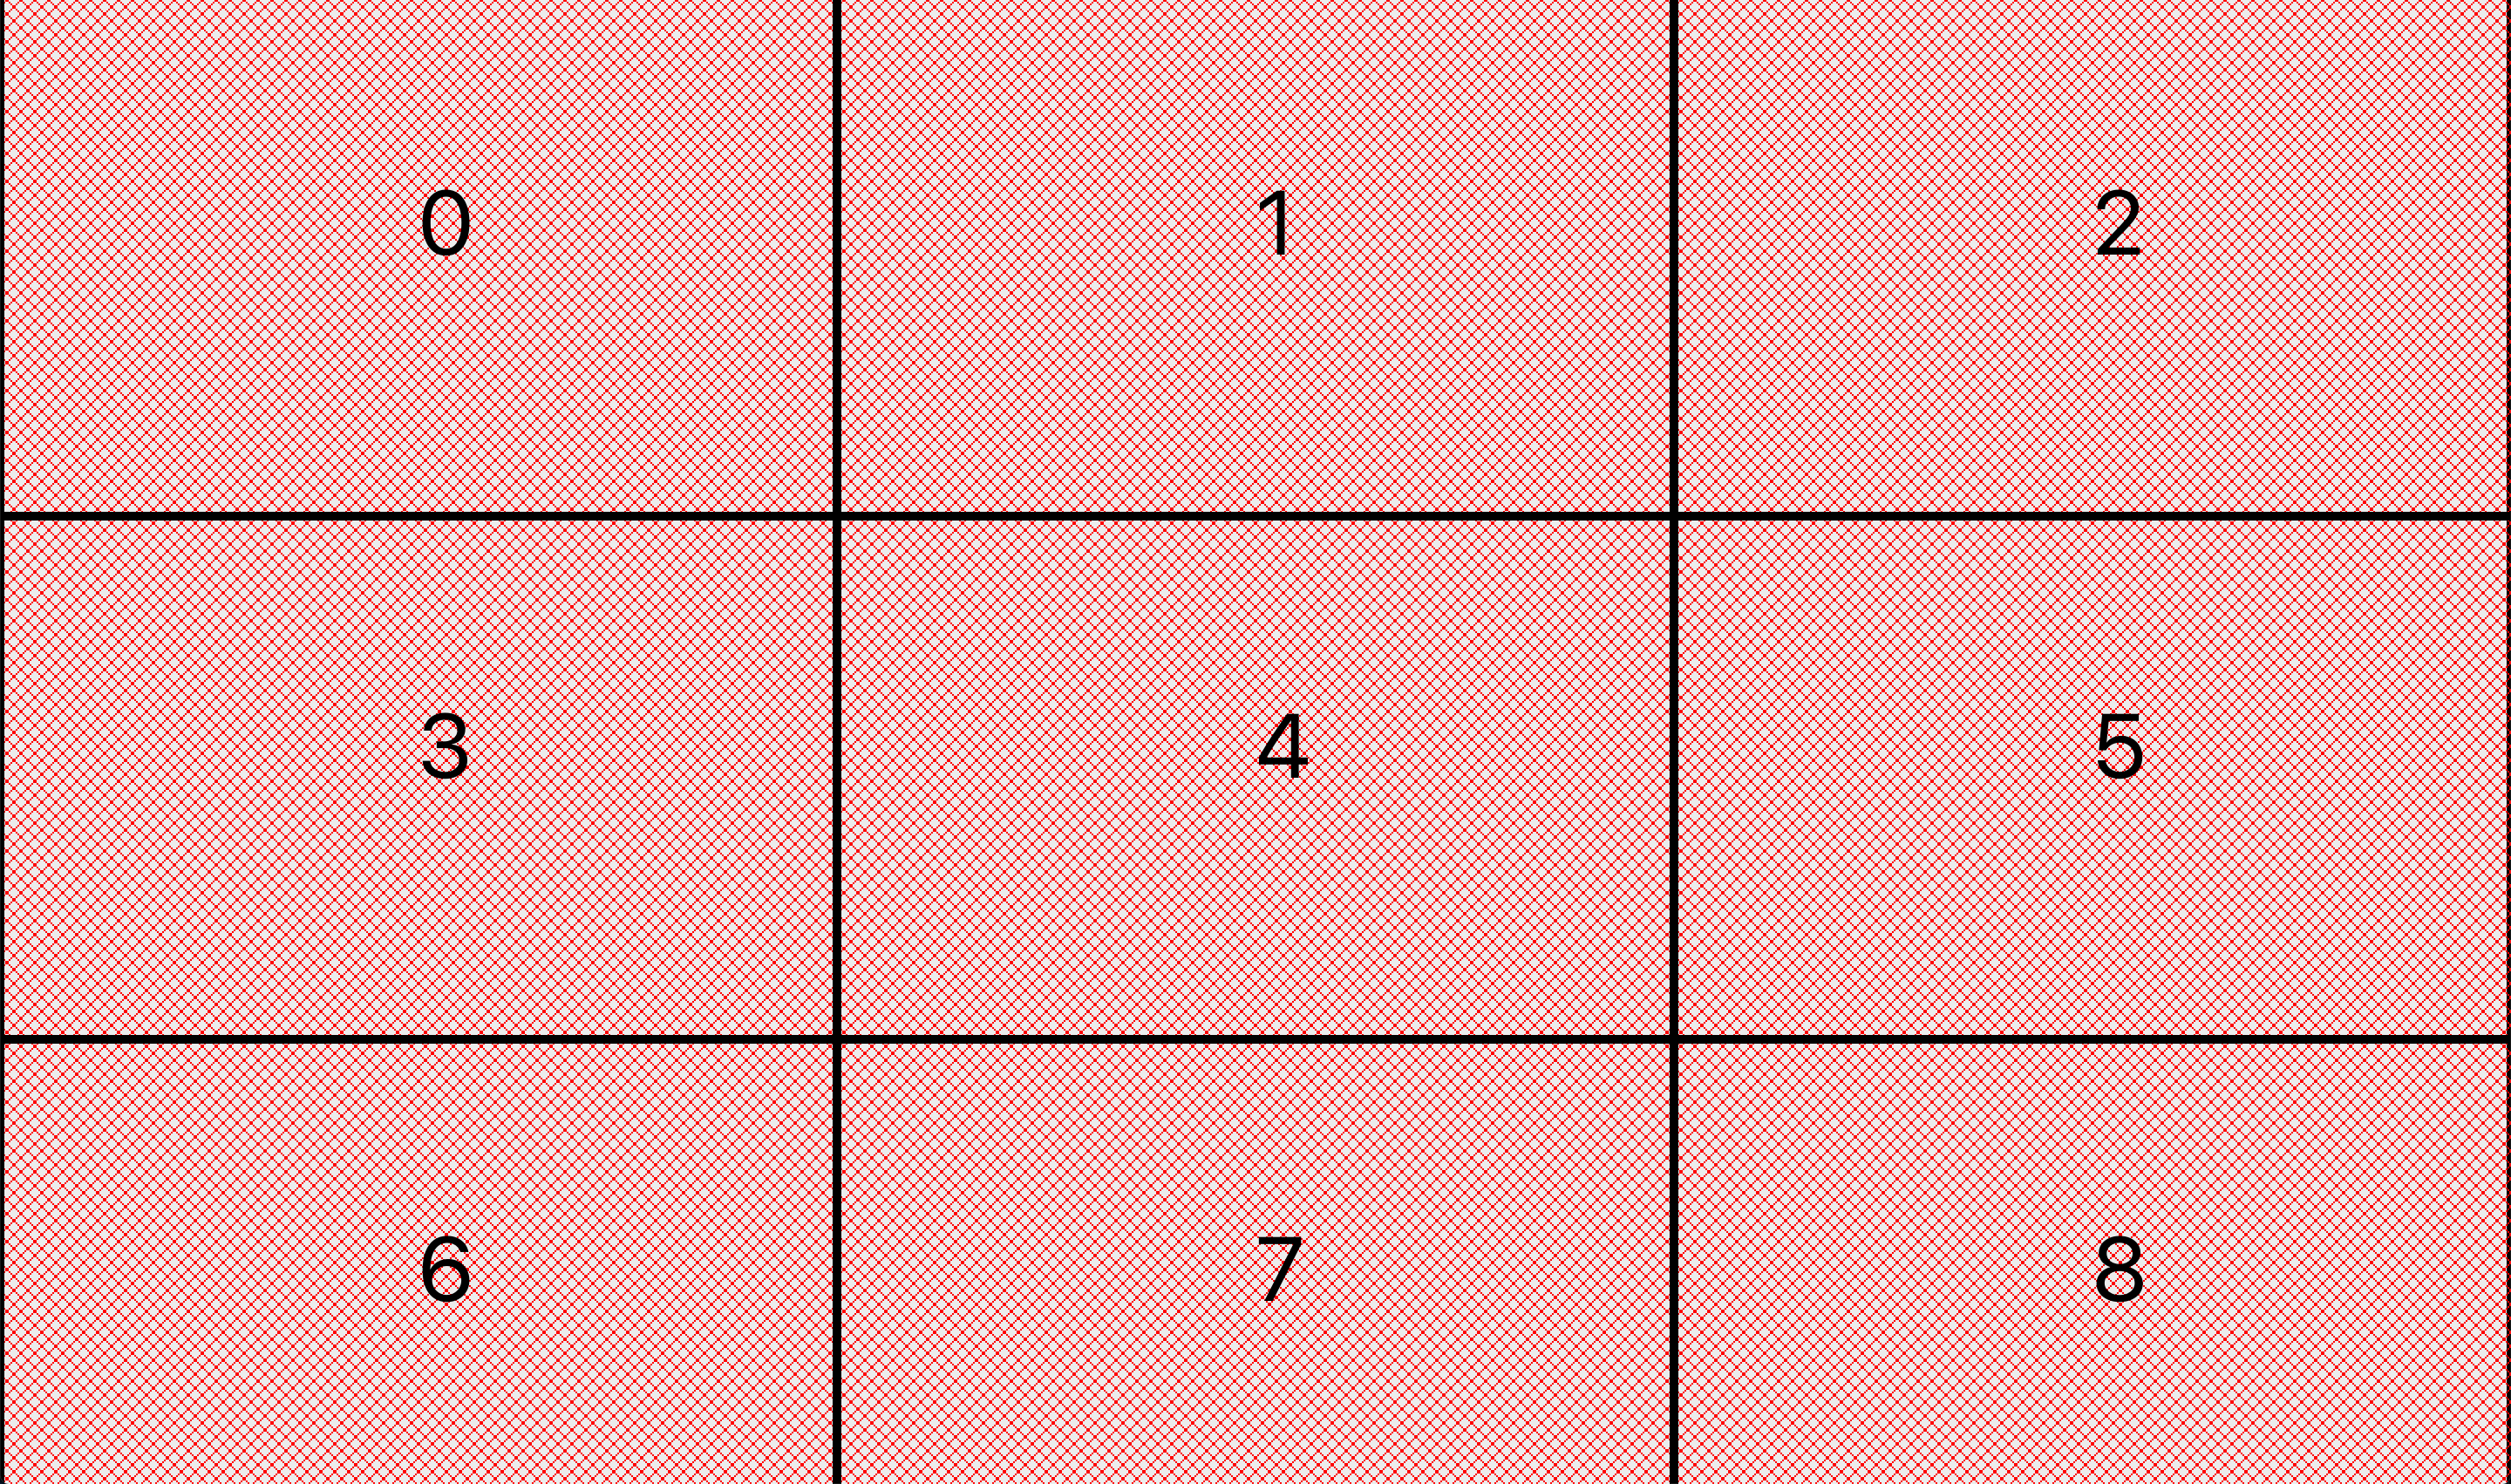
\includegraphics[width=0.32\textwidth]{grid_3_3.png}
    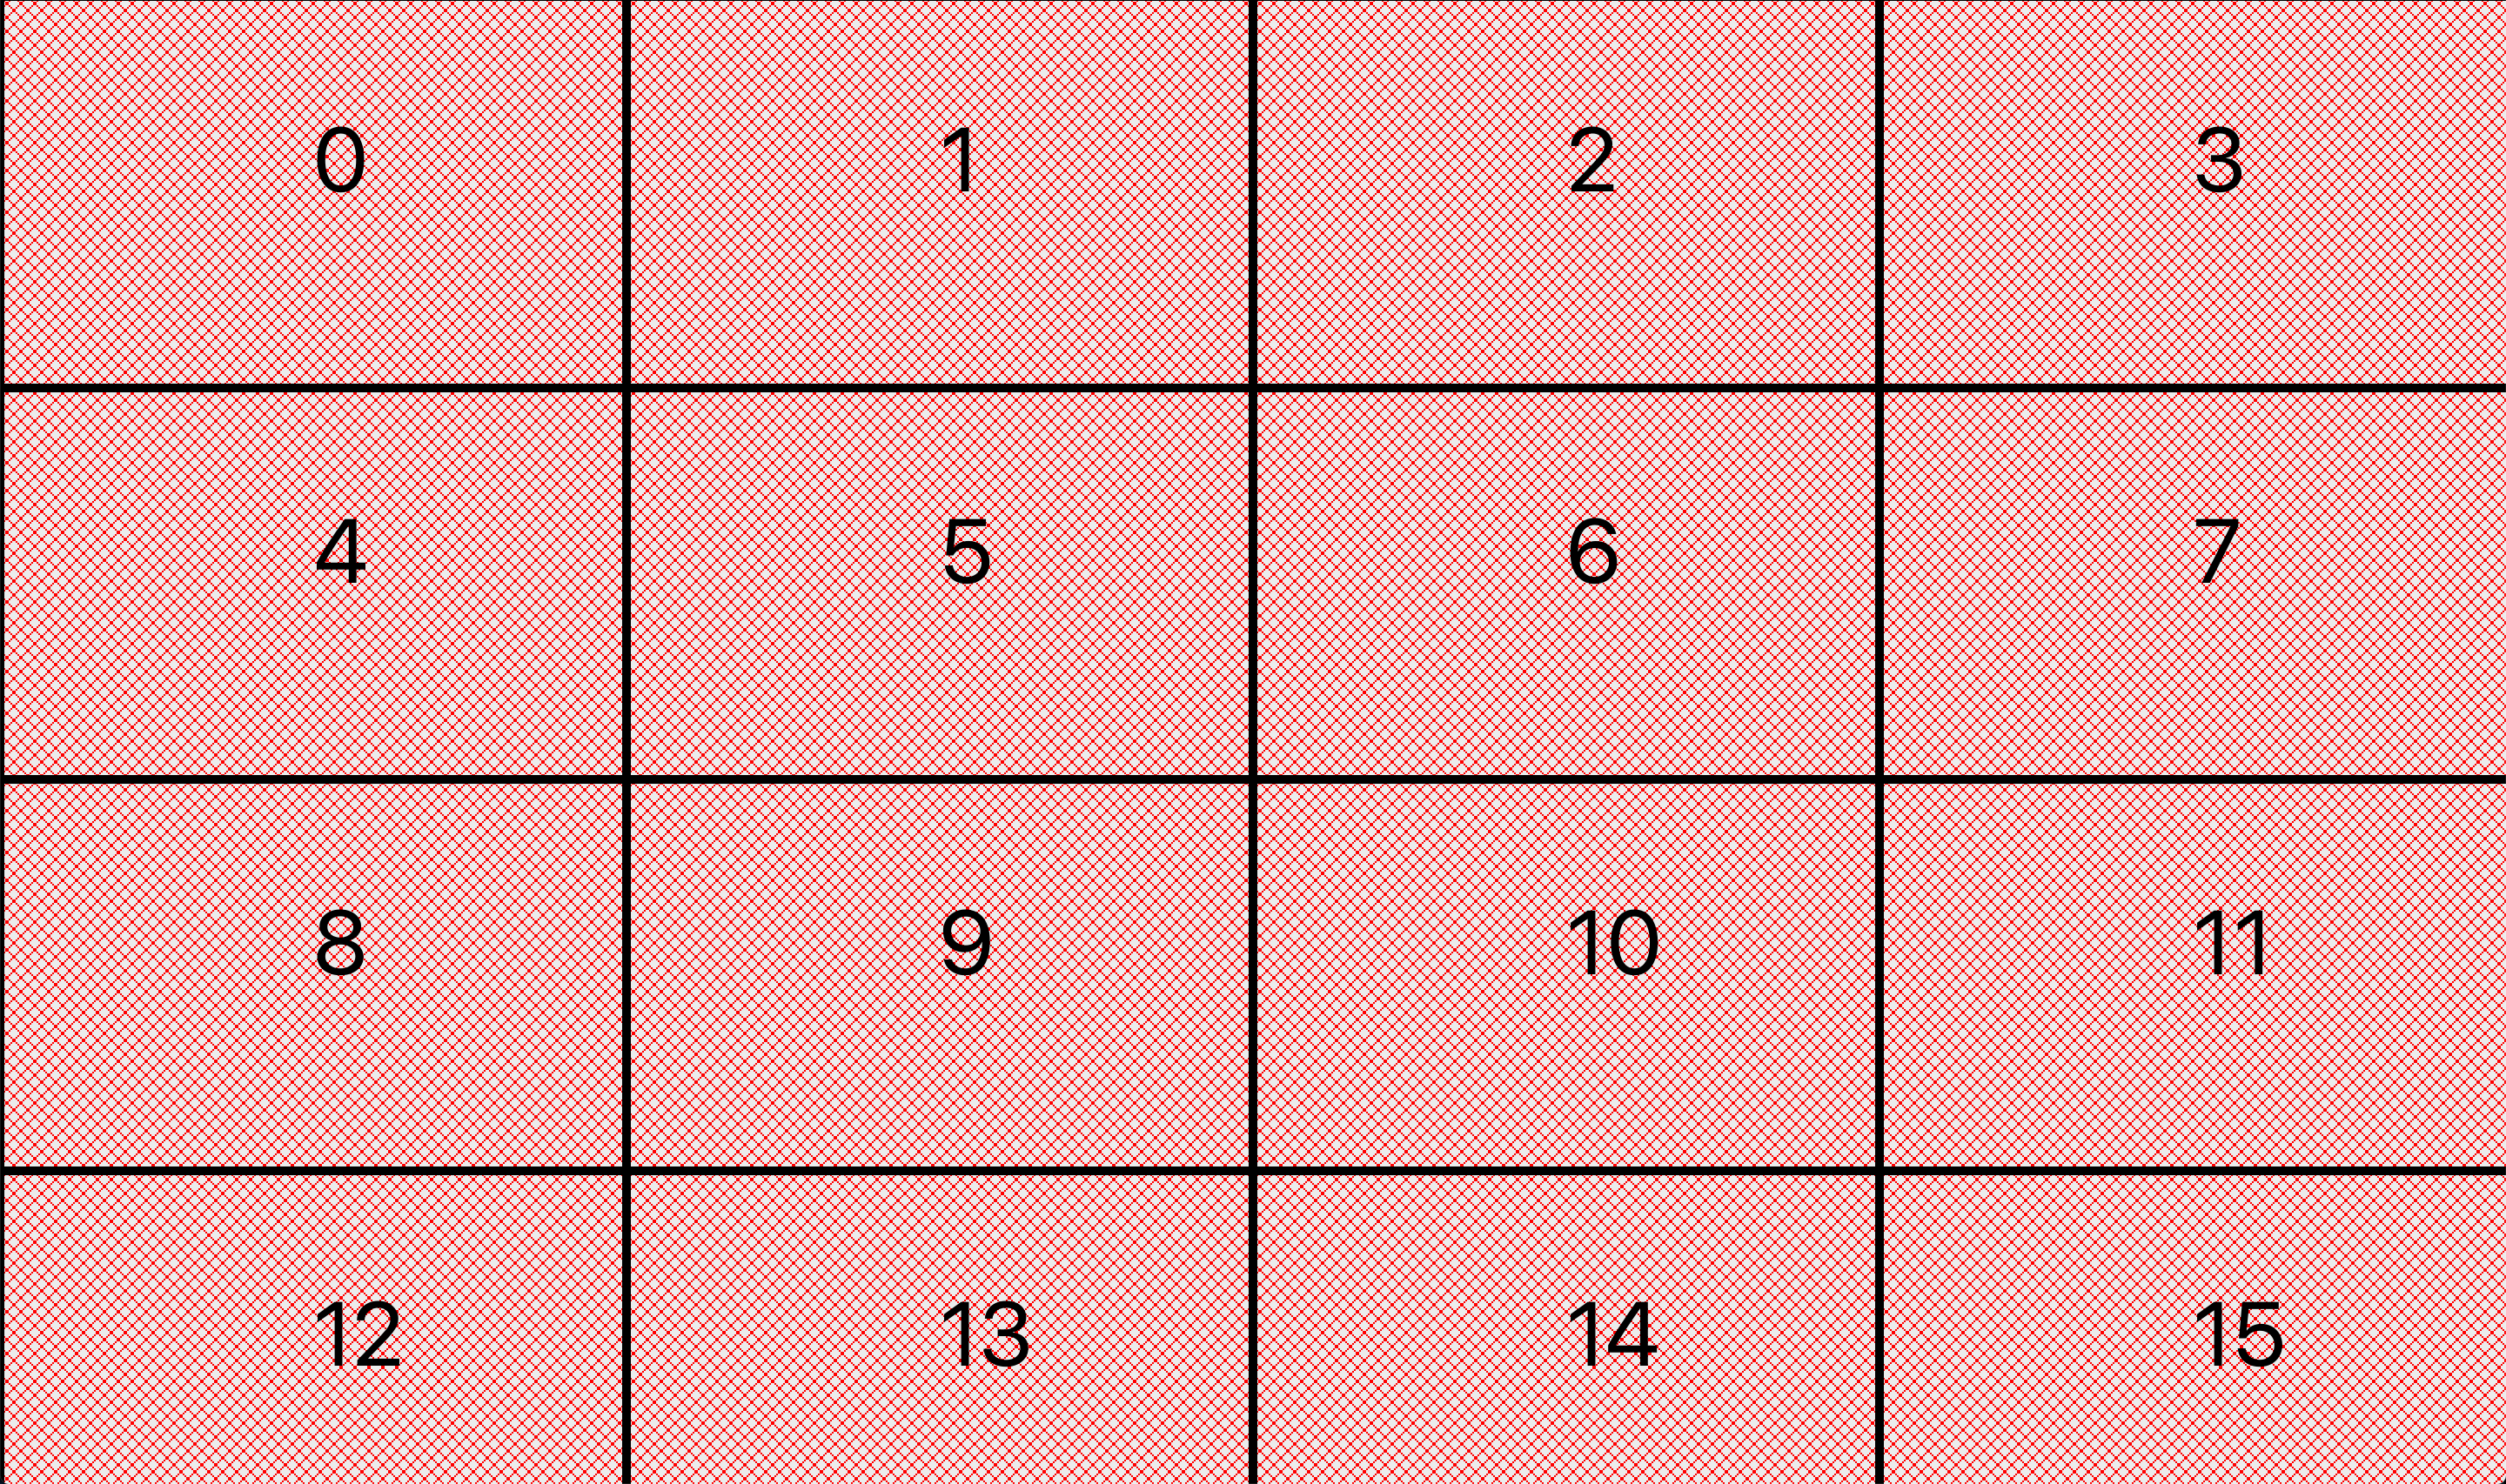
\includegraphics[width=0.32\textwidth]{grid_4_4.png}
    \caption{Exemple de grile plasate pe ecran}
    \label{grid-example}
\end{figure}

Așadar, mulțimea $I$ de mai sus va fi alcătuită din imagini alea utilizatorului, iar mulțimea $O$ va conține, spre exemplu, numărul celulei pe care o privea utilizatorul în imaginea respectivă.
Mulțimea $O$ este discretă și finită, așadar problema inițială este una de \emph{clasificare}.
Vom considera că pentru orice imagine din mulțimea $I$ nu conține imagini în care utilizatorul nu se uita la ecran.

Prima parte a problemei se traduce, așadar, astfel: dându-se o imagine cu utilizatorul privind ecranul, să se calculeze numărul celulei (în funcție de grila folosită) pe care utilizatorul o privește.
A doua parte a problemei ridică următoarea întrebare: cum putem simula funcționalitățile unui mouse doar prin gesturi ale feței?
Cum asigurăm o mișcare fluidă a cursorului spre o ``zonă țintă'', dar în același timp cursorul să rămână fix atunci când utilizatorul doar dorește să privească ceva de pe ecran sau să efectueze un click stânga/dreapta?

% \subsection{Neuronul Artificial}

% Înainte de a analiza arhitecturi de învățare profundă mai sofisticate, trebuie să aruncăm o privire rapidă asupra neuronului artificial.
% Pe scurt, este un model formal, simplificat al unui neuron biologic.
% Ne poate ajuta să realizăm \emph{clasificare binară} folosind următoarea formulă:
% $$
% y = \varphi (w * x + b)
% $$

% În formula de mai sus, $x$ este un vector de valori reale, reprezentând datele de intrare, iar $w$ este un vector de valori reale denumit \emph{vectorul ponderilor} (în engleză \emph{weights}) și $b$ este \emph{parțialitatea} (în engleză \emph{bias-ul}).
% Produsul $w * x$ reprezintă produsul scalar și este egal cu $w * x = \sum _{i=1}^{n}w_{i}x_{i}$, $n$ fiind lungimea vectorului $x$.


% Rezultatul clasificării este dat de $\varphi$, denumit \emph{funcție de activare}.
% Daca aceasta se comportă ca un prag, o limită, un \emph{threshold}, atunci funcția de activare se va traduce într-o clasificare binară, cu rezultat $0$ sau $1$.
% Putem folosi și $\varphi(x) = x$, ecuație care ne poate ajuta la rezolvarea problemelor de tip \emph{regresie liniară}.

% \begin{figure}[h]
%     \centering
%     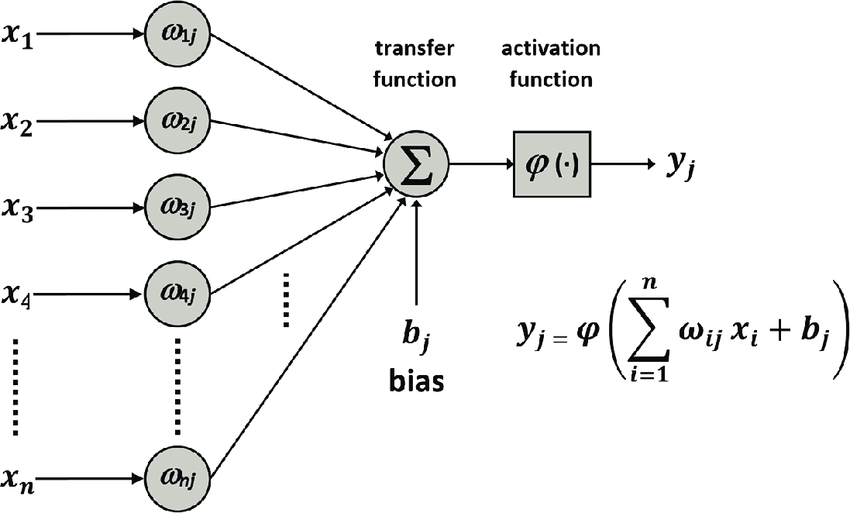
\includegraphics[width=\textwidth]{artificial_neuron.png}
%     \caption{Algoritmul perceptron, bazat pe neuronul artificial. Imagine preluată de pe site-ul \href{https://www.researchgate.net/figure/Scheme-of-a-perceptron-A-nonlinear-activation-function-BULLET-is-applied-to-the_fig3_315788933}{ResearchGate}}
% \end{figure}


% \subsection{Rețele neuronale}

% ``Calul de bătaie'' pentru problemele de Viziune Computerizată este Rețeaua Neuronală Artificială.
% Ea este, dupa cum sugerează și numele, compusă din mai multi neuroni artificiali, distribuiți pe mai multe \emph{straturi}.

% \begin{figure}[H]
%     \centering
%     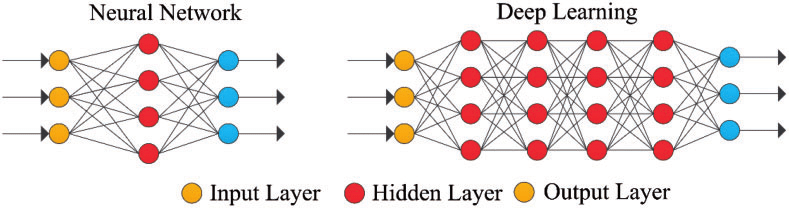
\includegraphics[width=\textwidth]{ann.png}
%     \caption{Structură generală a unei rețele neuronale. Imagine preluată de pe site-ul \href{https://www.researchgate.net/figure/Deep-learning-diagram_fig5_323784695}{ResearchGate}}
% \end{figure}

\section{Strategie}

\subsection{Obținerea datelor de antrenament}
Primul pas spre rezolvarea problemei este \emph{colectarea datelor de antrenament}.
Este foarte bine cunoscut că un algoritm de Învățare Automată este pe atât de bun pe cât sunt datele pe care i le furnizăm.
Acestea sunt incredibil de importante, așa că m-am concentrat pe a dezvolta niște modalități facile de a aduna o mulțime consistentă de date.

O altă etapă esențială este \emph{procesarea de date}.
Aceasta se preocupă cu simplificarea și curățarea setului de date, cu eliminarea instanțelor de antrenament care sunt inutile și cu extragerea exclusiv a informațiilor care sunt de folos și cu înlăturarea a ceea ce rămâne.
Opțional, în această etapă se mai realizează și diferite transformări pentru a aduce datele dintr-o formă neprelucrată într-o formă convenabilă algoritmilor pe care îi folosim.

\subsection{Predicția zonei de privire}
Următorul pas a fost cel de antrenare și de dezvoltare a unui model matematic capabil să prezică zona de privire a utilizatorului.
Pentru acest lucru m-am concentrat pe a studia \emph{rețeaua neuronală} care este ``calul de bătaie'' pentru problemele de Viziune Computerizată.

Un tip special de rețea neuronală este \emph{Rețeaua Neuronală Artificială} (\emph{Multilayer Perceptron Network}).
Ea este, dupa cum sugerează și numele, compusă din mai multi neuroni artificiali, distribuiți pe mai multe \emph{straturi}.
Am folosit această arhitectură ca un punct de pornire spre a rezolva problema și ca un prim experiment.

\begin{figure}[ht]
    \centering
    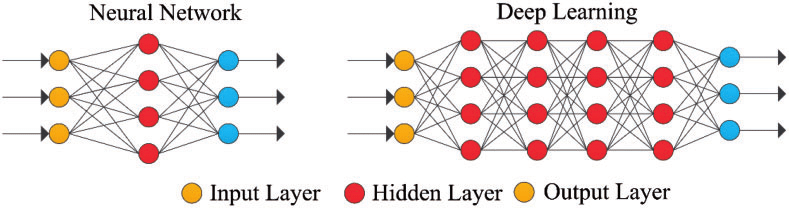
\includegraphics[width=\textwidth]{ann.png}
    \caption{Structură generală a unei rețele neuronale. Imagine preluată de pe site-ul \href{https://www.researchgate.net/figure/Deep-learning-diagram_fig5_323784695}{ResearchGate}}
\end{figure}

Folosind acest tip de rețea, am încercat să ating cel mai important obiectiv al acestei lucrări al licenței, și anume de a prezice aproximativ zona în care se uită utilizatorul, pentru a putea deplasa cursorul în acea zonă.
Din experimentele efectuate, această arhitectură a rezultat într-o primă soluție promițătoare, fiind capabilă să urmărească, într-o anumită măsura, privirea utilizatorului.

Apoi a urmat studierea și aplicarea \emph{rețelelor neuronale convoluționale}, o arhitectură de bază pentru multe metode ``state of the art'' pentru problemele din domeniul Viziunii Computerizate.
Cu ajutorul acestora, urmărirea ochilor a devenit mai robustă și mai puțin sensibilă la diferențele dintre imagini, precum lumină sau poziționare.

\subsection{Simularea funcționalităților mouse-ului}
Având un model care poate satisface nevoia de mai sus, de urmărire a ochilor, am analizat apoi cum pot simula efectiv funcționalitatea unui mouse.
Pentru aceasta, am analizat modalități de a folosi reperele faciale\ref{figure:facial-landmarks} pentru a folosi gesturi ale feței și a simula aceste funcționalități.
Soluția a constat în a folosi gesturi precum închiderea unui ochi și gestul de deschidere a gurii.

\subsection{Cercetare și analizare a bibliotecilor folosite}
În lucrarea de licență am folosit diverse biblioteci printre care și \lstinline{dlib}, pe care am folosit-o pentru a identifica reperele faciale ale utilizatorului.
Am fost curios despre cum anume funcționează această bibliotecă și am făcut un mic experiment în care am încercat să reconstruiesc funcționalitatea acestei librării.